%% This document gives an example on how to use the ntnumasterthesis
%% LaTeX document class.

%% Use short name MACS, MIS, CIMET, MTDMT, MIXD or MIS  
%% Language english or norsk
%% b5paper with oneside or twoside, you can set A4 if you want but you submit in b5

%% If you want print with the heading material on a4 paper you can use this format
%% \documentclass[MACS,english,a4paper,oneside,12pt]{ntnuthesis/ntnuthesis}

%% with the change to using DAIM we have a new option. include DAIM after english below removes the front page material so that you can then submit in the DAIM system. If you are wanting the front material remove DAIM and make sure you fill in the DaimData.tex file.
\documentclass[MIT,english]{ntnuthesis/ntnuthesis}

\usepackage[T1]{fontenc}
\usepackage[utf8]{inputenc}     % For utf8 encoded .tex files allows norwegian characters in the files. This can be dangerous if you change to a differnt editor.
%\usepackage[pdftex]{graphicx, hyperref}   % For cross references in pdf
\usepackage{graphicx}
\usepackage{hyperref}   % For cross references in pdf


\usepackage{color}              % For colouring text 
\hypersetup{colorlinks=true,     
		linkcolor=blue,          % color of internal links (change box color with linkbordercolor)
    citecolor=blue,        % color of links to bibliography
    filecolor=blue,      % color of file links
    urlcolor=blue           % color of external links
		}
\usepackage{csvsimple}  % for simple table reading and display
\usepackage{url}
\usepackage{booktabs}
\usepackage{gnuplottex} %miktex option if using miktex on windows
\usepackage{rotating}

\definecolor{darkgreen}{rgb}{0,0.5,0}
\definecolor{darkred}{rgb}{0.5,0.0,0}

\lstset{        basicstyle=\ttfamily,
                keywordstyle=\color{blue}\ttfamily,
                stringstyle=\color{darkred}\ttfamily,
                commentstyle=\color{darkgreen}\ttfamily,
}


%Typesetting of C++ but not always stable in titles etc...
\newcommand{\CPP}[0]{{C\nolinebreak[4]\hspace{-.1em}\raisebox{.1ex}{\small\bf +\hspace{-.1em}+\ }}}

%\usepackage[table]{xcolor}% http://ctan.org/pkg/xcolor
%\usepackage[nomessages]{fp}
%\newlength{\maxbarlen}


\newcommand\databar[3][gray!20]{%
  \FPeval\result{round(#3/#2:4)}%
  \rlap{\textcolor{#1}{\hspace*{\dimexpr-\tabcolsep+.5\arrayrulewidth}%
        \rule[-.05\ht\strutbox]{\result\maxbarlen}{.95\ht\strutbox}}}%
  \makebox[\dimexpr\maxbarlen-2\tabcolsep+\arrayrulewidth][r]{#3}}



\newcommand{\com}[1]{{\color{red}#1}} % supervisor comment
%\renewcommand{\com}[1]{} %remove starting % to remove supervisor comments
% This will appear in text \com{Lecturers comment} and be visible unless you uncomment
% the renewcommand line.

\newcommand{\todo}[1]{{\color{green}#1}} % items to do
%\renewcommand{\todo}[1]{} %remove starting % to remove items to do

\newcommand{\n}[1]{{\color{blue}#1}} % other comment
%\renewcommand{\n}[1]{} %remove starting % to remove notes

\newcommand{\dn}[1]{} % add the d to a note to say that you have finished with it.





% Set to true ONLY if using Harvard citation style
\newboolean{HarvardCitations}
\setboolean{HarvardCitations}{false} % false for computer science, true for interaction design and harvard style


\ifthenelse{\boolean{HarvardCitations}}{%
	\usepackage{natbib} % for Harvard names as citations.
}{%
	\usepackage[numbers]{natbib} % for Vancouver numbers in bibliography
}

\newcommand{\q}[1]{\leavevmode\marginpar{\small\em #1}}
\renewcommand{\q}[1]{}


\begin{document}

% for students submitting in the DAIM system this information will not be used.
% their is an option for DAIM submission which removes this information and checks it is B5.
% Removing the DAIM option on the document type will use this material.

\setthesistitle{Supporting Facilitation for Collaborative Learning in Mixed Reality (Working title)}
\setthesisshorttitle{Supporting Facilitation of Collaborative Learning in Mixed Reality} % a short version for the page headers if your normal title is too long to fit
\setthesisauthor{Stian Torjussen \& Jonas J. Husebø}


\setthesissupervisor{Prof. Monica Divitini \& Assoc. Prof. Ekaterina Prasolova-Førland}
\setthesissupervisorB{Assoc. Prof. Simon Mcallum}

%\setthesissupervisorB{Prof. Smart Guy}  % if you have a second supervisor add it like this


\nmtkeywords{Thesis, Latex, Template, IMT}
%\nmtdesc{This is the short description of a masters thesis}


\setthesisdate{22-06-2018}
\setthesisyear{2018}


%for CIMET theses you need to see all of these as well

%\setthesiscampus{Gj\o{}vik}
%\setthesisHostInstitution{\NTNU}
%\setthesisHostInstitution{University of Eastern Finland}
%\setthesisHostInstitution{Universit\'e Jean Monnet Saint-Etienne}

%\setthesisjuryA{} %jury names
%\setthesisjuryB{} %jury names
%\setthesisjuryC{} %jury names
%\setthesisjuryD{} %jury names


 % this is the file which contains all the details about your thesis
\makefrontpages % make the frontpages
%this is the intro to the thesis
%\thesistitlepage % make the ordinary titlepage
\hypersetup{pageanchor=false}
%\include{summary}

\chapter*{Preface}
Here, you give a brief introduction to your work. What it is (e.g., a Master's thesis in AIMT at NTNU, when it was carried out (e.g., during the autumn semester of 2021). If the project has been carried out with a company, you should mention this and also describe the cooperation with the company. You may also describe how the idea to the project was brought up.

You should also specify the assumed background of the readers of this report (who are you writing for).\\[2cm]

%\begin{center}
%\thesiscampus, 
\thesisdate \\[1pc]
\\[1pc]
%\thesisauthor
%\end{center}

\chapter*{Acknowledgment}
I would like to thank the following persons for their great help during \ldots

If the project has been carried out in cooperation with an external partner (e.g., a company), you should acknowledge the contribution and give thanks to the involved persons.

You should also acknowledge the contributions made by your supervisor(s).

\begin{flushright}
O.N.\\[1pc]
(Your initials)
\end{flushright} 

\chapter*{Abstract}

\hypersetup{pageanchor=false}



\tableofcontents

\hypersetup{pageanchor=true}

% Comment with a percent to remove figures or tables:
\listoffigures
\listoftables

\chapter{Introduction}
With the new rise of Virtual- and Augmented Reality technologies, devices like HTC Vive, Facebook's Oculus, and Microsoft's Hololense and Immersive Headsets have revolutionized the way we see and interact with digital information. These technologies have great potential, not only in entertainment, but for educational and collaboration purposes as well.

Virtual- and Augmented reality have primarily been used for entertainment in the fledgling years of their resurgence. Since Oculus stated that the Rift was primarily for gaming\cite{OculusMarkZuckerberg}, and HTC's partner, Valve, is one of the biggest names in the games industry\cite{ValveBigName}, the initial focus of the new Virtual reality Devices was clear. Even Augmented Reality technology was made popular by applications like Snapchat\cite{Snapchat} filters and the hugely popular Pokemon Go\cite{PokemonGo}.

Entertainment might be a reason for their initial success, there has also been applications of Virtual- and Augmented Reality outside of entertainment, like helping norwegian children to learn math\cite{innomag2017} or helping apprentices learn building systems\cite{Nordbohus2017}. These applications show that this kind of technology maybe has an even greater purpose outside of entertainment. With Microsoft's focus on Mixed Reality, giving a platform where Virtual Reality applications and Augmented Reality applications can work together, we wish to explore this technology in the setting of NTNU's Experts in Teamwork course.

\com{EIT should be described in much more detail in INtro, background and when connected to the requirements. 
1.Use official course information 'Guide for students in Experts in Teamwork 2017/2018' What are the learning goals you want to support? The motivation for introducing Mixed reality is that the use of LA that something that was probably not supported well enough in pure VR?
Also this is something nobody tried before. 
Describe also more explicit own experience with Gjøvik EiT spring 2017, identifying what EiT activities were supported in VR and what not. How this led to RQ?}


    
    \section{EiT VR Village}
        \subsection{What is EiT?}
        Experts in Teamwork(EiT) is a compulsory subject for Master students at NTNU. There are about 80 villages, each with its unique village theme. The general theme for the villages are problem areas from society and working life. In each village, students are divided into groups and are to define their own project related to the village theme.\cite{EiTAbout}
        
        The point of EiT is for students to develop interdisciplinary teamwork skills. By composing each EiT village of students from a wide range of disciplines, each student will learn how to work together in interdisciplinary groups. There is also a focus on reflection of one's own contribution in a team, and reflection on the team altogether.\cite{EiTAbout}
    
        \subsection{VR/AR for learning and training}
        This thesis has a strong connection to the EiT village "Virtual and Augmented Reality for Learning and Training". This village already had most of the required resources in place for the students to use, and the course description and goal of the village aligns with our motivation for exploring the possibilities in this field.
        
        On NTNU's page about the village (Translated to English):
        \emph{"Virtual and augmented reality (VR/AR) have had an explosive development the last years. This opens up big opportunities in an educational context. For example, safely and easily experience highly realistic educational situations that is not easily accessible in real life, like exploring the seafloor, burning buildings, or war zones. With this technology the students get access to visualizations and simulations that can contribute to a better understanding of syllabus and to better acquiring of skills, e.g. in a virtual lab or operation room.}
        
        \emph{Virtual reality also opens up new opportunities for remote education were students can work together in a virtual hospital or cooperate with students at NTNU Gjøvik and Ålesund. There are being developed games like Pokemon GO to give an introduction to local history. VR/AR can be used in adult education for everything from emergency response training and training of neurosurgeons to work training under direction from NAV. Virtual reality is also used for therapy and medical treatment, e.g. for mental and physical training and stimuli, for disabled people and the elderly."} \cite{EiTVRLandsby}
    
        \subsection{Our Experience}
        Both authors attended the EiT village "Virtual and Augmented Reality for Learning and Training" during the spring semester of 2017. During this semester we got to experience first hand some of the cutting edge technologies related to virtual and augmented reality. E.g. being able to try the Hololens, a very new and expensive device, making it a rare opportunity. Experiencing and developing for these technologies during the course is the main reason we chose this theme for our thesis.
        
        During the course, one of the authors was working on a project that consisted of expanding on a virtual reality collaboration application called IVR-Connection. This application was also at the same time expanded upon by two other groups linked to the EiT village. One of which were located in Gjøvik. The three group worked together on testing and expanding on IVR-Connection by having weekly meetings within the application. Each week some selected participants from each group would enter the virtual world and give status reports, share ideas and test each others solutions. This had great potential for being a productive way of collaborating across large geographical distances.
        
        It turned out however that more often than not it ended up being more work than value. This was partially because there was some technological difficulties with the application and the devices, but mostly because we just were not used to collaborating in a virtual environment. In EiT when a group is not performing optimally, a facilitator can step in and help them achieve greater efficiency. In virtual reality however this proved to be a little bit more challenging. The facilitator had a hard time getting an adequate overview over the collaborative situation in the virtual world, and because he was not co-present in the virtual space, it was also hard for him to relay feedback effectively. Since facilitation had a great effect on our groups efficiency outside of virtual reality, there is precedence for exploring the possibilities for expanding the collaboration application with internal support for facilitation.
        
    \section{Four Campuses One Reality}
    % Something about the vision and idea behind this initiative
    It's about connection Gløs, Draggis, Gjøvik og Ålesund through VR.
    Notes: NTNU merge, VR EiT village, Joint effort between Gjøvik and Trondheim, Idea to connect the campuses through VR, the idea is that, given the right tools, this should work better than using VOIP and video, its all about presence and the tools that can be given to you in a virtual world. \cite{4C1R}
    

\chapter{Background}
\label{chap:background}
% Explain what this chapter is all about!
In this chapter we will give an introduction to background for our master thesis as well as the tools, technology and previous research that made it all possible. 

    \section{EiT VR Village}
        \subsection{What is EiT?}
        Experts in Teamwork(EiT) is a compulsory subject for Master students at NTNU. There are about 80 villages, each with its unique village theme. The general theme for the villages are problem areas from society and working life. In each village, students are divided into groups and are to define their own project related to the village theme.\cite{EiTAbout}
        
        The point of EiT is for students to develop interdisciplinary teamwork skills. By composing each EiT village of students from a wide range of disciplines, each student will learn how to work together in interdisciplinary groups. There is also a focus on reflection of one's own contribution in a team, and reflection on the team altogether.\cite{EiTAbout}
    
        \subsection{VR/AR for learning and training}
        This thesis has a strong connection to the EiT village "Virtual and Augmented Reality for Learning and Training". This village already had most of the required resources in place for the students to use, and the course description and goal of the village aligns with our motivation for exploring the possibilities in this field.
        
        On NTNU's page about the village (Translated to English): \emph{"Virtual and augmented reality (VR/AR) have had an explosive development the last years. This opens up big opportunities in an educational context. For example, safely and easily experience highly realistic educational situations that is not easily accessible in real life, like exploring the seafloor, burning buildings, or war zones. With this technology the students get access to visualizations and simulations that can contribute to a better understanding of syllabus and to better acquiring of skills, e.g. in a virtual lab or operation room.}
        
        \emph{Virtual reality also opens up new opportunities for remote education were students can work together in a virtual hospital or cooperate with students at NTNU Gjøvik and Ålesund. There are being developed games like Pokemon GO to give an introduction to local history. VR/AR can be used in adult education for everything from emergency response training and training of neurosurgeons to work training under direction from NAV. Virtual reality is also used for therapy and medical treatment, e.g. for mental and physical training and stimuli, for disabled people and the elderly."} \cite{EiTVRLandsby}
        
    \section{NTNU Dragvoll VR Lab}

    \section{Concepts}
    
        \subsection{Virtuality Continuum}
        The Virtuality Continuum(VC), as shown in Figure \ref{fig:virtualcontinuum}. \emph{"Is a concept which relates the mixture of classes of objects presented in any particular display situation."}\cite{Milgram1994} This article, "\emph{A Taxonomy of Mixed Reality Visual Displays}" by Paul Milgram and Fumio Kishino\cite{Milgram1994} introduces the concept of a "virtuality continuum" to describe the range of environments shown on any particular display. The articles focus on the taxonomy of Mixed Reality displays, and is also one of the earliest adapters of the concept of Mixed Reality.
        \begin{figure}[!ht]
            \centering
            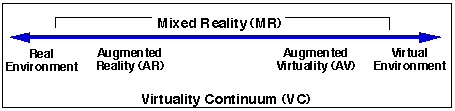
\includegraphics[scale=1]{figures/virtualcontinuum.png}
            \caption{Simplified representation of a "virtuality continuum".\cite{Milgram1994}}
            \label{fig:virtualcontinuum}
        \end{figure}
        
        \subsubsection{Virtual Reality}
        Using Milgram's and Kishinos's description of Virtual Reality(VR) from their paper.\cite{Milgram1994} VR is the concept of a virtual space where the user is fully immersed in a virtual world, usually through a Head Mounted Display(HMD). This means that the environment, and everything the user sees and interacts with is completely synthetic. The environment can emulate the real world and seem like reality, be it fiction or otherwise; or this virtual environment might be a world where our physical laws do not apply. On the virtuality continuum, as shown in Figure \ref{fig:virtualcontinuum}, this type of environment resides on the furthest extreme, opposite the real environment.
    
        \subsubsection{Augmented Reality}
        Augmented Reality(AR) is the concept of a real environment with digital elements superimposed, enhancing the users perception of reality.This is achieved by rendering these digital "\emph{holograms}" on a transparent display which the user sees through(e.g. Microsoft's Hololens or Magic Leap. The same effect can also be achieved by superimposing the digital elements onto video captured by a camera in real-time.
        
        \subsubsection{Mixed Reality}
        As shown in Figure \ref{fig:virtualcontinuum}, a Mixed Reality(MR) display can reside anywhere between the extremes of the virtuality continuum\cite{Milgram1994}. The technology has moved on since 1994, when the paper by Kishino and Milgram was published. \emph{"Since then, the application of mixed reality goes beyond displays but also includes environmental input, spatial sound, and location."}\cite{wdc-mr}
        
        Microsoft, especially, has expanded on the application of Mixed Reality. And in the article "What is mixed reality?"\cite{wdc-mr}. MR is described like this: \emph{"Most mobile phones on the market today have little to no environmental understanding capabilities. Thus the experiences they offer cannot mix between physical and digital realities. The experiences that overlay graphics on video streams of the physical world are augmented reality, and the experiences that occlude your view to present a digital experience are virtual reality. As you can see, the experiences enabled between these two extremes is mixed reality"}\cite{wdc-mr}. This spectrum is found in Figure \ref{fig:mrspectrum}
        
        \begin{figure}[!ht]
            \centering
            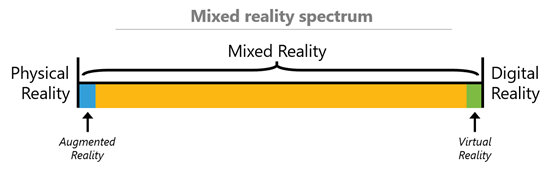
\includegraphics[scale=1]{figures/mixedrealityspectrum.png}
            \caption{The Mixed Reality Spectrum\cite{wdc-mr}}
            \label{fig:mrspectrum}
        \end{figure}
        
        In Figure \ref{fig:mrdevicetypes} the two main device types that deliver Windows Mixed Reality is listed. These are: Holographic devices, which has the ability to place digital content in the real world;\cite{wdc-mr} and Immersive devices, which has the ability to hide the physical world and replace it with a digital experience.\cite{wdc-mr} 
        \begin{figure}[!ht]
            \centering
            
\includegraphics[scale=1]{figures/mixedrealityspectrumdevicetypes.png}
            \caption{Mixed reality device types.\cite{wdc-mr}}
            \label{fig:mrdevicetypes}
        \end{figure}
        
        \subsection{Holograms}
        
        \subsection{Immersion} % Research and definition of what immersion means in the context of VR
        Immersion in relation to computer games is "used to describe the degree of involvement with a game" \cite{Brown2004}. In the paper by Brown in 2014 he defines three different levels of immersion: Engagement, engrossment and total immersion. Each level has its own barriers that needs to be removed for that level of immersion to be possible. Entering a higher level of immersion is correlated with having a higher level of concentration and focus \cite{Jennett2008}. For IVR-Connection this is one of the concepts that can give the user an advantage over collaborating in "real life".
        
        \subsection{Presence} % Research and definition of what presence means in the context of VR
        Jennet et al. presents two different perspectives on the definition of presence \cite{Jennett2008}. The first has basis in the rationalistic tradition, and defines presence as a psychological sense of being in a virtual environment \cite{Slater1994}. With this perspective the level of presence has to be evaluated through user feedback. The other bases itself on the Heideggerian/Gibsonian metaphysics, and relates presence to the ability of "successfully supported action in the environment" \cite{Zahorik1998}. With this perspective presence can be evaluated through empirical means. Presence and immersion have a lot in common and are often used interchangeably. However, Jennet et al. argues that presence is a state of mind, while immersion is an experience in time \cite{Jennett2008}. With this distinction presence and immersion are allowed to overlap, but it is also possible to have one without the other.
        
        \todo{Explain "Ready-In-Hand" and "throwness". This relates to what presence means for mixed reality}
    
    \section{Technology}
    % What technology are we using.
    In this section we will cover the technology that made everything possible. This master is based on cutting edge technology from Microsoft and Unity.
    
        \subsection{Universal Windows Platform}
        % About UWP. What is it and why we use it
        Universal Windows Platform (UWP) provides a common app platform for every device that runs Windows 10. An UWP app is written in C++ /WinRT or C++ /CX and has access to the Win32 APIs that are part of the UWP. These Win32 APIs are implemented by all Windows 10 devices.\cite{wdc-UWP} Examples of devices running Windows 10 are: Desktop computers, phones, XBOX and Hololens.
        
        \subsection{Mixed Reality Toolkit}
        % What is it and why we use it
        \emph{"The Mixed Reality Toolkit is a collection of scripts and components intended to accelerate development of applications targeting Microsoft HoloLens and Windows Mixed Reality headsets. The project is aimed at reducing barriers to entry to create mixed reality applications and contribute back to the community as we all grow."}\cite{MRToolkitReadme}
    
        \subsection{Unity}
        % What is it and why we use it
        Unity is a game engine for creating 2D, 3D, VR, AR and MR games and apps. It has its own graphics engine and a full-featured editor that enables you to create games, and deliver your content to virtually any media or device. Unity also features services like cloud building, multiplayer network, version control and analytics. Unity is also at the forefront of the growing VR market. An estimated 90\% of Samsung Gear VR games and 53\% of Oculus Rift (games at launch) were[sic] Made With Unity. \cite{UnityAbout}
        
        \subsection{Unreal}
        One of the oldest and most used game engines (20 years). Been used by multiple award winning AAA games. Written in C++ and is highly optimized for PC, VR and Mobile platforms.
        Visual coding in C++ using blueprints.
    
        \subsection{Hololens}
        The Hololens is Microsoft's holographic device. Using inside-out tracking, it is a fully mobile head mounted device running Windows 10. It has full six-degrees of freedom movement and uses a see-through display to render the "\emph{holograms}".
    
        \subsection{Immersive Headsets}
        Under the Mixed Reality Moniker, the Immersive Headsets are VR headsets that uses built-in inside-out tracking. With no need for external sensors, and only one cable for connection with the PC; One can enjoy VR from anywhere. Headsets are provided by multiple different big name retailers, all providing their own designs and solutions for the platform.
    
    \section{Related Work}
        
        \subsection{IVR-Connection}
        % About this program and how it fits in with the vision and idea from 4C1R
        Program made by Nicklas to test cooperation in VR.
        
        \subsection{Virtual Reality Spectating}
        
        \subsection{Medical Procedural Training in Virtual Reality}
 % includes latex files from the same directory
\chapter{Theory}

    \section{Collaboration}

    \section{Collaborating in Mixed Reality}
    This section will contain research on the benefits and drawbacks of collaborating in Mixed Reality. As well as the definition of what it means to do so.
    
    \section{Collocated Collaboration}
    
    \section{Remote Collaboration}
    
    \section{Collaborative Learning} % Research on benefits and drawbacks for using VR for collaboration?
    This section will contain research on the benefits and drawbacks of collaborating in VR. As well as the definition of what it means to do so.
    
    \section{Project Based Learning}
\chapter{Methodology} % could be called Methodology or methods or any filename 
 % \chapter{Results} % could be results
\chapter{Phase 1}
    \section{Exploration}
    In the beginning of the first phase time was spent looking for ways to integrate Hololens into the already existing IVR-Connection application. To accomplish this, we had to look at the code of IVR-Connection and browse online for already existing solutions for Hololens in Unreal.
    
        \subsection{IVR-Connection}
        IVR-Connection was developed in 2016?, and used Unreal version 14.0, in relation to VR technology and especially Windows Mixed Reality, this could be considered as an old version of Unreal Engine. This meant that IVR-Connection needed an engine version update for it to be best able to support the newest VR technology, e.g. Hololens. We were tasked by our supervisors and stakeholders to update IVR-Connection to establish a stable baseline, a 1.0 release of IVR-Connection. This baseline was to act as the new official version that every other student working on the application would use. The aim was set at Unreal Engine release 4.18, as it provide a lot of new features and support for VR technology, making it a good version for a stable baseline for a VR application. Unfortunately it had no official support for Windows Mixed Reality and Hololens.
        
        \com{Connect much stronger to EiT needs and learning goals!}
        
        \subsection{Hololens Support}
        The best way to support Hololens, is to support UWP. Unreal engine did not natively support UWP at the time, but Microsoft were working on a branch of Unreal that did. This branch also had a sub branch called dev\_MixedReality which added support for Windows Mixed Reality. In addition there was a plugin called ProteusVR that added templates and blueprints for Hololens to this branch. ProteusVR had just reached version 1.0 and the lead developer promised to rapidly release updates as Windows' mixed reality branch evolved. The mixed reality sub branch did however not support Unreal engine 4.18 at the time. Since the priority for IVR-Connection was to support HTC Vive and be on the cutting edge of VR features, updating to Unreal engine 4.18 got prioritized over merging to the new Microsoft branch. In addition both the Microsoft branch and ProteusVR were both actively being developed. This meant that there was a chance for them both to catch up with 4.18 while we worked on the stable baseline for IVR-Connection. Thus Hololens support was set on hold until IVR-Connection 1.0 was finished.
        
        \subsection{VR Lab Space}
        
        \com{Connect this to EiT learning goals (several students in VR together!)}
        Early January, the VR lab at NTNU Dragvoll finished construction. The lab consisted of four Vive headsets in different booths in the same room, each with its own set of base stations. The VR booths had an open design: With one of the side open and openings at the top of the walls. This caused the the base stations' infrared light to bleed into the adjacent booths. This introduced issues with the spatial tracking for some of the Vive headsets. Several solutions were applied to fix this issue: 
        \begin{enumerate}
            \item Configure the base station in such a way that they could only one base station with a compatible setting.
            \item Using sync cables to ensure that the correct pair of base stations synced to each other.
            \item Stacking pieces of cardboard along the upper wall to block the light leaking over the wall.
            \item Putting cardboard boxes with one side open over the base stations to limit the angle that they were sending light.
            \item Using blinds to block any light entering through an opening in the side wall of one of the booths.
        \end{enumerate}
        
        The first fix was supposed to stop the base stations from syncing with the wrong base stations, this solution was not perfectly consistent however. The second fix was applied to address this issue, and this time the base stations consistently synced correctly to each other. The third fix stopped the light from leaking over the wall, effectively eliminating light leaks for some of the VR booths. Light bleeding from one booth to the other meant that the Vive headset would sometimes get confused about its spatial orientation. This had averse effects for the person wearing the headset, as the world would move around erratically, often causing nausea or dizziness. To further assure that no light was escaping over the wall, fix 4 was applied. Fix 5 had to be applied to one of the booths due to a hole in one of the side walls. With all the base stations syncing correctly and the light leaks fixed, the Vive headsets were now operating predictably. The issues experienced with having multiple Vive setups in the same room will according to HTC Vive's website be addressed with the 2.0 version of SteamVR and the 2.0 version of the base stations. % Some pictures for visualization, small, grouped side by side, in two rows if needed. Find a nice place to cite for 2.0. Best I found was the buy page, can we cite that? https://enterprise.vive.com/eu/
 
    \section{Implementation} % Fixing and updating to 4.18.
    The strategy for updating IVR-Connection to Unreal engine version 4.18 was carried out in two steps. Since 4.18 didn't get released before 23rd of October 2017, the first step was to update to 4.17. This was to be able to address as many deprecation issues as possible before 4.18 released, making the transition a little bit smoother. After 4.18 was released IVR-Connection was updated again, bringing it up to date with the newest VR features Unreal could offer. % Ref 4.18 release date blog post containing list of new features? https://www.unrealengine.com/en-US/blog/unreal-engine-4-18-released
        
        \subsection{Plugins}
        There were two plugins attached to the original version of IVR-Connection: VR Expansion and that other one. VR Expansion Released updates for 4.17 and eventually 4.18, so we did not need to modify anything using this plugin. That other one one the other hand seemed to be dead, and had not released any updates in a while. We therefore removed the plugin and rewrote the blueprints that had been using it. This was done with native functions within the Unreal engine. % Find name and exact date for last version of the other plugin.
        
        \subsection{Image Loading}
        The blueprints for loading and sharing images used features from the removed plugin which had no equal within the Unreal engine. Loading images had also previously proved to freeze the main thread while the image was being loaded. The solution to both these issues were finding a small piece of code that allowed for loading the images asynchronous to the main thread. % Ref code source + picture or code snippet?
    
    
    \section{Evaluation} % Internal Evaluation, What made us change
    The evaluation of phase 1 consisted of 1 survey with 26 respondents and an internal evaluation regarding Hololens and Unreal.
    
        \subsection{Survey} % UKA questionnaire
        The survey were a part of a stand at UKA technology conference, were people could come and test IVR-Connection for Vive before filling it out. The goal was to get an idea of what people think about using VR for collaboration and learning, as well as to get an overview of what features the respondents deemed most important in such a scenario.
        
        Of the total 26 respondents, 46.2\% had tried VR a few times before while only 11.5\% had tried it many times, which leaves 42.3\% that had never tried VR before that day. Because the definition of many and a few can vary from person to person, it only makes sense to make a distinction between those who had tried VR before, and those that had not.
        
        The survey showed that interacting together in VR can be an exciting and engaging experience, since all respondents agreed to this. Which is reflected in their excitement about the idea of using this for collaboration and lectures in the future. In other words, the survey confirmed that the concept of IVR-Connection was worth continuing on.
        
        24 of the total 26 respondents said that they felt a strong or some sense of presence in the VR world, but only 11 agreed that it was easy to follow what the others were doing. When observing the respondents trying IVR-Connection, an emerging trend was that they lost track of the other users when they were teleporting. This might indicate that the application needs some features for tracking the other users location, e.g. adding spatial sounds and/or particle trails when people are teleporting.
        
        % TODO: avsnitt om features
        
        \subsection{Hololens} % Lacking Hololens support for Unreal
        By the end of the first phase the mixed reality branch of Unreal developed by Microsoft were still stuck in 4.16, and ProteusVR had not seen any activity in 4 months. This meant that we either had to switch back to Unreal 4.16 or find another way of using Hololens for a collaborative environment.
        
        Switching back to 4.16 and using Microsoft's Unreal branch, could make it unnecessarily complicated for the other students working on the project. As well as limiting development when it comes to supporting the newest standards and VR hardware optimally. Thus we decided not to continue down the path to add Hololens support for IVR-Connection for Vive.
        
        Instead we directed our attention towards Unity. Unity offered support for the newest in VR hardware and was Microsoft's own recommended engine for developing 3D applications for Hololens and Windows Mixed Reality. To further accelerate development Microsoft had also started working on a plugin, called Holotoolkit. This tool was developed as an open source project and had a high level of activity, which meant relatively frequent updates. In addition making our own software, meant more freedom to explore in the directions we wanted. Thus we opted to take the concept of IVR-Connection and implement it with Hololens support in Unity. % https://docs.microsoft.com/en-us/windows/mixed-reality/development-overview
\chapter{Phase 2}
    \section{Requirements}
    For the second phase, requirements where elicited based on the results of the UKA questionnaire from phase 1 combined with personal experiences with collaboration in VR. This section lists these requirements.
    
    \com{Should be explained much better how the requirements are derived from the EiT learning goals, the need for facilitating and theory, e.g. immersion and social presence}
    
        \subsection{F1 - VR/MR? Collaboration Space}
        The user should be able to enter a collaborative space. The collaborative space should have the following features:
        \begin{enumerate}
            \item The space must feel roomy and spacious at the same time.
            \item The space must function as a collaborative space, e.g not be too fancy or captivating.  "supporting sense of presence?"
            \item The space must be easy to navigate, e.g. have objects placed about to give you a sense of depth.
        \end{enumerate}
        
        \subsection{F2 - Avatar}
        The user should have an avatar that represents him/her in the virtual space. The avatar should have the following features:
        \begin{enumerate}
            \item The avatar should follow the movement of the player.Identity? Social presence
            \item There should be 2 different avatars. One for immersed headsets and one for the hololens.
        \end{enumerate}
        
        \subsection{F3 - Movement}
        The user should be able to move around in the virtual space. The movement should be governed by the following features:
        \begin{enumerate}
            \item The user must be able to walk around in the virtual environment by walking around in the real world.
            \item The user must be able to teleport using a controller.
        \end{enumerate}
        
        \subsection{F4 - Multiplayer}
        The user should be able to connect to other users. The multiplayer system should contain the following features:
        \begin{enumerate}
            \item The user should be able to host a session from any supported device.
            \item The user should be able to search for active sessions created by other users.
            \item The user should be able to join an active session.
            \item The user should be able to disconnect from the currently active session.
        \end{enumerate}
        
        \subsection{F5 - Drawing}
        The user should be able to communicate and visualize through drawing. The drawing should be governed by the following features:
        \begin{enumerate}
            \item The user should be able to draw on a surface.
            \item The user should be able to draw in the air in 3 dimensions.
            \item The user should be able to choose a color to draw with.
            \item The user should be able to erase what has been drawn.
        \end{enumerate}
        
        \subsection{F6 - Media Sharing}
        The user should be able to share media like video and images to other users. The sharing of media should be governed by the following features:
        \begin{enumerate}
            \item The user should be able to open a sharing menu.
            \item From the sharing menu the user should be able to share media with the other users.
            \item When shared, a game object representing the media should be spawned in the virtual space.
            \item The user should be able to move the spawned game object.
        \end{enumerate}
        
        \subsection{F7 - Voice Chat}
        The user should be able to communicate by using a voice chat. The voice chat should contain the following features:
        \begin{enumerate}
            \item The user should be able to speak to other users using a microphone.
            \item When a user speaks there should be an indication of it in the virtual space.
            \item The voice chat should be activated as soon as a user hosts a session.
        \end{enumerate}
        
        \subsection{F8 - Interactable Objects}
        The user should be able to play around with physically intractable objects in the virtual space. These objects should have the following features:
        \begin{enumerate}
            \item The user should be able to pick up the object.
            \item The user should be able to throw the object.
            \item When thrown the object should maintain momentum according to the physical laws of the virtual space.
        \end{enumerate}
        
        \subsection{F9 - Hololens Spectating}
        The user should be able to spectate the virtual space by using a Hololens. Using the Hololens should be governed by the following features:
        \begin{enumerate}
            \item The user should be able to move the virtual collaborative space.
            \item The collaborative space should be moved relative to the real world, e.g. can be place on a table or on the floor.
            \item When using the Hololens the virtual space should appear small enough to fit on a table.
        \end{enumerate}
    
    \section{Implementation} % Implementation of IVR-Connection in Unity. Based on requirements.
    For the second phase not all requirements where met. Only the most essential features to complete a proof of concept test where implemented. The rest of this section will list and describe these features.
    
        \subsection{Collaboration Space}
        The collaboration space is the playing area where the immersed players can move around and interact with each other and the environment. It is designed to meet requirement F1. It has some boxes placed about to make it feel less empty, and a big whiteboard where the immersed players can draw. Attached to gameobject is a LevelLogic script. It contains the logic for how the different headset types should spawn and scale the collaboration space. % Add picture. Not much more to say?
        
        \subsection{Avatar}
        The avatar consists of a model with a PlayerController script attached, and was designed to meet requirement F2 and F3. The PlayerController script contains all the logic for how the player can interact with the virtual world. Due to lack of 3D modelling skills and time, the model for the avatar were taken from Microsoft's 250 Mixed Reality tutorial. The model is under the MIT licence. % Pictures and ref to the tutorial
    
        \subsection{Match Maker}
        The match maker is based on Unity's match making system using UNET and HoloToolkit's example menu. The match maker contains logic for creating, searching for and joining matches and was extended to be able to transmit room data from Hololens to Hololens. The UI follows the player around and anchors around the bottom of the viewport. It only supported creating and joining matches. The join button where for testing purposes hard coded to search for matches, and then join the first match it found. The match maker was implemented to meet requirement F4. % Pictures
        
        \subsection{Drawing}
        Drawing was implemented by giving the player a pen and a palette. The pen is used to draw on the whiteboard in the collaboration space. This is done by pointing the colored tip towards the whiteboard and drag it around, just like in the real world. The palette is used to change color. The player can change the color of the pen by touching the colors on the palette with the tip of the pen.  % Pictures + something about the code?
        
        \subsection{Hololens Spectating}
        Joining or creating a session while using a Hololens gives you a birds eye view of the collaboration space. Upon joining or creating a session, the collaboration space will spawn relative to you and your physical environment. The player can move the collaboration space by doing a tap gesture to pick it up, and another tap gesture to place it down again. The collaboration space will align with the spatial data gathered by the Hololens. If someone with an immersed headset joins the session, they will appear in the collaboration space. The Hololens will thus be able to observe the interactions of those with the immersed headsets. Hololens spectating was implemented according to requirement F9.
    
    \section{Evaluation}
    The evaluation of phase 2 consisted of one user test with 7 EiT students and 5 facilitators followed by a focus group session with 2 of the facilitators, and a survey for all 12 of them.
    Due to some bugs in the network code, the multiplayer and cooperation aspect fell out of focus, and only the individual features where properly tested. This means that only the concept of the application and the individual features were evaluated.
    
    \com{5 facilitators here but 2 in the next sections? Confusing, explain the settings better, in a separate subsection!}
    
        \subsection{Survey} % Summary of survey data.
        This subsection will contain a summery of the survey data.
        % Purpose
        
        % VR collab and outside
        
        % Physical lab space
        
        % EiT course, not relevant?
        
        % Vive Application
        
        % Mixed Reality Application
        
        % Facilitators
        
        \subsection{Mixed Reality Application Concept} % Summary of interview. Relevant to Mixed Reality.
        % TODO: Connect with requirements.
        The same two facilitators didn't get to do a full test in the Mixed Reality version due to some technical difficulties. But both looked at the concept and a demo with the Hololens. The paragraphs below is a summary of what was said and discussed.
        
        The avatar for the Hololens was too big and intrusive. It is important that the facilitators doesn't take all the attention of the room, but rather acts as a fly on the wall. At least when you are observing. When you are about to give feedback, having a feature that temporarily makes you able to acquire the students attention would be nice. Like for example descending down into their world with a gesture or another in-game indicator that make them understand that you want their attention. It is important that this is comfortable for the students.
        
        The facilitators suggested that it would be nice to be able to write on the whiteboard while spectating as Hololens. By adding this feature the facilitator could explain both verbally and visually, and interact with what the students have written themselves. Especially useful for doing EiT exercises.
        
        Even less body language to observe in this version. The application had only avatars with a moving body and a rotating head. No indicator for speech and no hands for gesticulating.
        
        The facilitators also suggested adding the ability to import documents and write on them. This to be able to implement some EiT form exercises into the application. One way to do this is by implementing the ability to import images and draw on them. Making the user able to mark of on forms and saving the result for inspection by the facilitators.
        
        \subsection{Vive Application} % Summary of interview. Relevant to Vive application
        % TODO: Connect with requirements.
        Was tested by two facilitators. One with and one without the Vive headset which both had pros and cons. The following paragraphs is a summary of what were said and discussed in this interview.
        
        The VR lab enabled one facilitator to watch the Trondheim side of the collaboration via the screens in the room. This required a lot of concentration and ended up being tiresome. It felt a little like watching TV and thus he felt more distant than usual when trying to facilitate. Watching through the participants eyes he only got to see what they were looking at, and trying to follow 4 screens looking for collaborative elements was hard. Especially since the level of body language he could read were limited, although he could see 3 of the participants in the room with him, their faces where obscured by the Vive headset. The hardware and equipment also posed limitations, especially on the Gjøvik side, since they only had one phone acting as a microphone. This generated a lot of noise, making it somewhat hard to follow conversations. The threshold for giving feedback and suggestions were higher, since his presence were only heard and not seen. The students completed an EiT exercises name "take space, give space". 
        
        \com{More details here!}
        
        Due to technical and software limitations this took a lot more time in VR than in the real world. Making it more effort than gain. He also noted that using Skype or another VOIP application with a video feed might have been more efficient for this type of exercises, at leas for this version of the IVR-Collaboration.
        
        The other facilitator tried facilitating with the Vive headset and found that using VR can be uncomfortable and nauseating. For example when the headset picks up signals from the wrong base station, it will get confused and throw you around in the world. She also pointed out that it was hard to pick up on body language and was missing facial expressions, as these are signs she usually picks up on when facilitating in the real world. She also experienced that the VR world had a lot of unrelated stimuli. There is always something more interesting to look at, especially the first times you try it. And since the audio is only in their head, the visual stimuli might at times take more of your focus than intended. In other words, it might be harder to pay attention to what people are saying.
        
        Approximately 70\% of communication comes from body language. And the body language the EiT students used were very different from what the facilitators had observed outside of VR. The facilitators speculated that this could be due to another group dynamic when collaborating with Gjøvik in contrast to internally with each other. They also speculated that it could be due to the anonymity of the session. Especially when someone is talking and not referring to anything in the world, the students tended to look at their hands or pay attention to something else, at least visually. Another factor might be that this is an application that is part of a test project that the EiT students didn't choose to use themselves. It has a lot of bugs and technical difficulties so the facilitators speculated that this could give them an "get it over with" mentality and make them not take it seriously.
        
        Avatars and anonymity can be good for racial and gender bias, as neither of them are visually visible in the application. The facilitators agreed that keeping this feature could be good for inclusion and equality. But that it is still important to be able to distinguish between the different participants, and that name tags can be a good candidate for this. The facilitators also agreed that the avatars should match the purpose. For example do not use animals or crazy outfits for a normal meeting session.
        
        Long session in VR can be tiresome and induce nausea for many different reason. One thing the facilitators noted was that they found it strange that the students decided to stand during whole length of the meeting. This might be due to you not being able to see the chair beside you inside the VR world.
        
        \subsection{Requirements} % F1 - 5 partially fulfilled, F6 - 8 not fulfilled, F9 almost fulfilled.
        Not all requirements were met for phase 2. Requirement F1, F2, F4 and F5 were partially met and F6 - F8 were not met at all. Requirement F9 was met, but lacked some specification that were added for phase 3, and requirement F3 was completely met. The rest of this section will briefly discuss the fulfillment of each requirement.
        
        For requirement F1 it was hard to determine if it was met or not. Requirement F1.1 and F1.2 were too unspecific and hard to understand what was actually required. Requirement F1.3 seems to have been met, since none of the test participants had any trouble navigating the environment. To test this case thoroughly, it would also be required to test the application with people less experienced with VR.
        
        The Avatar followed the player as describe in requirement F2.1, but did not have a separate avatar for Hololens as required by F2.2. This was due to F2.2 being of low priority when critical bugs were still present right before the test was conducted. Requirement F2 also lacked the specification for the two different avatars.
        
        The requirement F3 were met. The player can move around by walking in the real world as describe by F3.1 and teleport using a controller as describe by F3.2. The player is thus able to move around in the virtual space.
        
        Multiplayer was very unstable for phase 2, but the requirements were almost met anyways due to lacking specifications for stability and long levity. These specification had to be added in phase 3 for a correct measure of working multiplayer functionality. Aside from that the requirements F4.1, F4.2, F4.3 were all completely met through the implemented match maker. Requirement F4.4 were however not met due to the lack of a disconnect feature, apart from forcibly closing the application by external means.
        
        The Drawing functionality almost met the requirements specified in F5. Through a pen and a palette the player were able to draw on a surface (the whiteboard) as specified by F5.1 and choose a color by using the palette as required by F5.3. To be able to erase what had been drawn and thus fulfilling requirement F5.4, the player could select the color white, which was the same white as the whiteboard. Drawing in 3D as described by F5.2 was not fulfilled and was also set to a low priority for phase 3. The render method used for drawing also caused a lot of frame rate drops for Hololens, thus requirements regarding performance had to be added for phase 3.
        
        Requirement F6 - F8 were, as mention earlier, not fulfilled at all. Mostly because these were giving a lower priority than the rest of the requirements. Requirement F6 describes sharing media. This feature were implemented through image sharing with limited functionality, but were left out because it was difficult and complex to use, and due to the lack of a proper UI implementation. Requirement F7 described voice chat. The voice chat functionality were given a lower priority due to the expected problems with limited bandwidth through Unity's network service, and because using a third-party software was just as viable. Requirement F8 described intractable objects and were given a low priority due to the low impact it would have on the completed product.
        
        Requirement F9 were met for phase 2. The player was able to spectate the virtual space by using the Hololens, as well as move the collaboration space relative to the real world as specified by requirement F9.1 and F9.2. The collaboration space fit on a table as describe by requirement F9.3, but the interviews revealed that it was to small to follow what the immersed players were doing. Thus further specifications were needed for in phase 3.
        
\chapter{Phase 3}
    \section{Updated Requirements} % Only write changes to requirements here. Alt title: Phase 2 Changes to Requirements.
    For phase 3 it was necessary to update the requirements from phase 2. The updated requirements are mainly based on the interviews with the facilitators. The updated requirements are listed in this section.
    
        \subsection{F1 - VR Collaboration Space} % Write about changes to the requirements, and then display them. Might make a table for requirements.
        No big changes were done to this requirement. F1.1 and F1.2 were rewritten to make more sense and be more precise, without changing the underlying meaning. The updated requirement is shown below.
        \newline\newline
        The user should be able to enter a collaborative space. he collaborative space should have the following features:
        \begin{enumerate}
            \item The space must not be too big, and at the same time it must be spacious enough to not feel cramped.
            \item The space must function as a collaborative space and not be too fancy or captivating, as this might draw attention away from the task at hand.
            \item The space must be easy to navigate, e.g. have objects placed about to give you a sense of depth.
        \end{enumerate}
        
        \subsection{F2 - Avatar}
        For the avatar two additional requirements were added to make a distinction between the avatar for Hololens and the avatar for immersed headsets. F2.3 describes the immersed avatar and F2.4 describes the Hololens avatar. The updated requirement is shown below.
        \newline\newline
        The user should have an avatar that represents him/her in the virtual space. The avatar should have the following features:
        \begin{enumerate}
            \item The avatar should follow the movement of the player.
            \item There should be 2 different avatars. One for immersed headsets and one for the hololens.
            \item The Immersed avatar should have a body, a head and two hands.
            \item The Hololens avatar only needs a head.
        \end{enumerate}
        
        \subsection{F3 - Movement}
        No changes were made to this requirement.
        
        \subsection{F4 - Multiplayer}
        For multiplayer two new requirements were added to specify the minimum requirements for the stability and capacity of a session. F4.5 describes stability and F4.6 describes capacity.
        \newline\newline
        The user should be able to connect to other users. The multiplayer system should contain the following features:
        \begin{enumerate}
            \item The user should be able to host a session from any supported device.
            \item The user should be able to search for active sessions created by other users.
            \item The user should be able to join an active session.
            \item The user should be able to disconnect from the currently active session.
            \item A session should be stable and optimized for sessions lasting 30 minutes or more.
            \item A session should support a minimum of 4 simultaneous users.
        \end{enumerate}
        
        \subsection{F5 - Drawing}
        For drawing one new requirement were added to specify how much impact drawing can be allowed to have on the frame rate.
        \newline\newline
        The user should be able to communicate and visualize through drawing. The drawing should be governed by the following features:
        \begin{enumerate}
            \item The user should be able to draw on a surface.
            \item The user should be able to draw in the air in 3 dimensions.
            \item The user should be able to choose a color to draw with.
            \item The user should be able to erase what has been drawn.
            \item Drawing should not lower the frame rate of the application with more than 10 frames.
        \end{enumerate}
        
        \subsection{F6 - Media Sharing}
        No changes were made to this requirement.
        
        \subsection{F7 - Voice Chat}
        No changes were made to this requirement.
        
        \subsection{F8 - Interactable Objects}
        No changes were made to this requirement.
        
        \subsection{F9 - Hololens Spectating}
        For Hololens spectating one requirement was updated and 3 were added. Requirement F9.3 were changed to reflect the new requirement F9.4. F9.4 describes the users ability to be able to scale the collaboration space. Requirements F9.5 and F9.6 describes a personal whiteboard for the Hololens spectator.
        \newline\newline
        The user should be able to spectate the virtual space by using a Hololens. Using the Hololens should be governed by the following features:
        \begin{enumerate}
            \item The user should be able to move the virtual collaborative space.
            \item The collaborative space should be moved relative to the real world, e.g. can be place on a table or on the floor.
            \item The starting scale of the collaborative space should appear small enough to fit on a table.
            \item The user should be able to scale the collaborative space.
            \item The user should have its own personal whiteboard that can be scaled and moved in the same manor as the collaborative space.
            \item The personal whiteboard should replicate what is drawn on the whiteboard in the collaborative space.
        \end{enumerate}
    
    
    \section{Implementation} % Improving IVR-Connection for Unity. Stability, features, optimization. Based on feedback and remaining unfulfilled requirements.
    During phase 3 improvements were made toward having a more stable and complete product based on the update requirements. This section lists the different features implemented and explains what was created and updated.
    
        \subsection{Collaboration Space}
        The collaboration was scaled to fit the height of the user better. To do this the overall height of the space were brought down and the width made a little smaller. On the scripting end, LevelLogic.cs now makes sure that both the scale and position of the space is synced relative to the avatars. This ensured that every player gets the same and correct state of the world.
        
        \subsection{Avatar}
        The Avatar were scaled to match the new scale of the collaboration space, and to fit better relating to the headset user and the ground. The goal of the new scale is to make it easier to feel immersed in the space. split into two different game objects. One for Hololens players and one for immersed headset players. This was to make it easier to develop individual features for the different hardware.
        
        The Hololens avatar is now a cloud in the sky. This was to make the spectator less intrusive to the once collaborating in the space, while at the same time being able to draw attention if needed. The cloud model were taken from Microsoft's 250 mixed reality tutorial.
        
        The immersed avatar now has a pair of hands in addition to the body and the head. The hands will follow the movement of the motion controllers used with the immersed headset. If no controllers are connected, the hands will be hidden. A speech indicator were also added to let the other players see when someone with an immersed headset is talking. The speech indicator consists of a red ball over the players head. The red ball will be visible when the player speaks, and hide itself otherwise.
        
        A name tag were added for both avatars. The name can be set in the menu before you join or create a session, and will hover above the players head. The name will help the players keep track of who's who. % Add some pictures of this.
    
        \subsection{Match Maker}
        The UI of the match maker were moved closer. This was to make it easier to read the labels on the buttons. A search button were added to let the player search for matches before joining. This was added to make the application ready to handle multiple sessions at the same time. When the player search for a match, any session found will be displayed above the buttons in a list. The player can then select the session and click join to join the selected session.
        
        The network code were optimized to send less data per second. This was needed due to the low bandwidth limit put in place by Unity's networking service. To accomplish this all networked messages were forced to only happen a certain amount per second. Ranging from a couple to 30 times per second. This still wasn't really enough to keep within the limits. To properly fix this issue, we would need to either start paying for Unity Pro and Unity's network service, or implement another network system. None of these options were really valid. Unity Pro and its network services costs a lot of money, and implementing a new network system would have taken more time than was available. In the end we chose to move on because the application now run just long enough to do a multiplayer test.
        
        \subsection{Drawing}
        Due to the network optimizations the drawing feature had to be tweaked. The drawing data that had to be synced between clients were reduced to the smallest possible type. This resulted in the color scheme for drawing now only supports 256 different colors, but for most practical purposes this should be enough to use the whiteboard effectively.
        
        The drawing process also had to be optimized due to limited processor power on the Hololens. To accomplish this the logic of applying draw data to the whiteboard texture were separated from the draw logic itself. Because applying data to a texture is a CPU heavy task, this allowed us to reduce the CPU load by applying data less often. With the immersed headsets this was not an issue and thus they could continue to apply data as fast as they were drawing, but for the Hololens the frequency were lowered to 10 times per second. 
        
        Lowering the frequency to 10 times per second, synced the drawings on the whiteboard frequently enough to effectively follow what the other players were drawing. It also reduced the load on the CPU significantly, but the spikes generated still caused low frame rates when run on the Hololens. The solution to this could be to use a shader for drawing on the whiteboard texture. A shader would move the work load from the CPU to GPU, which is much more optimized to handle such tasks. Even though this might have been a good solution, we lacked shader competence and time to learn and implement it properly. Resulting in any further optimization effort to be put on hold. In the mean time the application could be streamed from the computer to the Hololens, effectively working around the issue.
        
        \subsection{Hololens Spectating}
        The scale of the world as the Hololens sees it were scaled up. This was to make it easier to follow what the immersed player where doing in the collaborations space. A bigger extra whiteboard that only the Hololens can see was also added. This whiteboard can be moved around and placed relative to the real world, just like the collaboration space. This new whiteboard replicates what is drawn on the original whiteboard. This is to make it easier for the Hololens user to see what is being drawn.
        
        Because of the issues with drawing and network service, the Hololens cannot effectively run the application on its own. A computer with Unity engine version 2017.2p1 and the source code from Git is needed. With Unity open you can stream the application to the Hololens while letting the computer do all the heavy lifting. At the same time the Hololens can still use gestures and gaze controls to interact with the application. Thus this work around let us test Hololens spectating without having to worry about limited hardware resources.
    
    \section{Evaluation} % This might get its own chapter
    The evaluation for phase three consisted of one user test with two VR experts and a facilitator, followed up by a focus group session. In the test the VR experts were told to cooperate to complete a drawing challenge while the facilitator observed and took notes of how they cooperated. The goal of the test was for the facilitator to evaluate if using Hololens for observing cooperation in VR gives any potential advantages when trying to facilitate.
        
        \subsection{Focus Group Feedback}
        % Hvem, hva og hvordan
        The focus group consisted of 3 participants; One EiT facilitator and two VR experts. The two VR experts were both master students at NTNU, and had been working with VR for 1.5 years. Where one of them had spent a year working with the Hololens. The facilitator also participated in the focus group for phase 2, and have had half a year of experience with VR and facilitating.
        
        The focus group were handled as a semi structured interview with open questions that everyone could answer and discuss. The goal was to evaluate if any improvements had been made since phase 2, and how the applications stacks against IVR-Connection for Vive or collaboration in real life. Especially in relation to facilitating. The rest of this section contains a summary of what was discussed during this focus group session.
        
        % Tegning er bedre
        The whole focus group agreed that the strongest feature implemented so far, was the drawing. They said that it was easy and intuitive to use, and that it was an improvement to the drawing system implemented for IVR-Connection for Vive. The only thing that they thought was confusing, was which button they had to press to activate drawing. One of the VR experts suggested that adding a controller scheme visualization could fix this issue. For the Hololens the facilitator said that it was now much easier to follow what was drawn on the whiteboard. This was mostly due to the addition of the personal larger whiteboard viewable for the Hololens user.
        
        % Immersion er bedre med sky og hender, er det ok å bli snakket til av en sky?
        Both the VR experts and the facilitator said that they felt immersed in the world. They all forgot about the outside world and focused only what was happening in the application. One of the VR experts stated that the cloud in the sky were less intrusive than the old Hololens avatar, making it less distracting. The others agreed. When asked about the new hands, one of the VR experts said that it made him feel more present because he was able to wave and make other simple hand gestures. He also mentioned that this feature could be improved by implementing even better hands. For example by adding a skeleton mesh and allow the player to open and close the hand, or point with only one finger extended. The same was true for the head of the avatar.  % Maybe add statement about animating the face and connect it with social presence.
        
        % Enkelere å se hva folk gjør, egen tavle hjelper, speechindicator og navn gjør det enkelt.
        The VR experts both agreed that it was easy to follow what the other were doing in the collaboration space. With the hands, speech indicator and a name tag, it was easy to grab attention when needed. They also added that they thought that the speech indicator and name tag would be especially helpful when collaborating with more people. The facilitator also agreed to all of this, but when using the Hololens the speech indicator and name tag was a little bit too small. The same issue was true for the hands. This meant that she had to move in close to clearly see who was talking and what gestures they were making. To fix this inconvenience the scale of the name tag, the speech indicator and the hands could be increased when using the Hololens.
        
        The facilitator stated that facilitating in MR is a lot different from facilitating in real life. She agreed that this was partially because you get less information about the subjects when you are facilitating MR, than you would if you were facilitating in real life. One of the biggest differences is the lack of advanced body language. She also added that although it is different and you get less information, it is still enough information to give feedback and facilitate cooperation. And added that it would probably most efficient if you were observing the subjects cooperate in real life and in MR.
        
        One thing that eased facilitating cooperation in VR, is the focus that comes with putting on a head mounted display and entering a virtual space with the sole purpose to collaborate. The facilitator meant that this makes it easier to facilitate, because almost everything that goes on in this space is related to collaboration. She also added that the Hololens comes with some advantages in relation to this phenomenon. First of all, the Hololens does not bring you, as a facilitator, completely away from the real world. This means that you can blend realities by observing the virtual space while taking notes in your notebook in the real world. There is also a certain familiarity to placing objects on a table and watching it from different angles. This makes it easy to use and gives you a lot of overview of what is happening. Which is a huge advantage for a facilitator.
        
        The facilitator also added that she felt that there was a lower threshold for giving feedback. The main reason for this was that she felt like a part of the virtual space when she was inhabiting the Hololens avatar. The VR experts agreed with there being a low threshold for starting a conversation, and added that the anonymity of the avatars might also be a factor to this. They all also agreed that another factor might be that they got to know each other before the test started. The facilitator added that getting to know each other might not factor in specifically on the threshold itself, but rather making everyone take each other more seriously.
        
        Even though the threshold for giving feedback were lower, the facilitator added that the current version of the application did not give her a way to get the immersed players' attention. With this she meant that there were no incentive for the immersed player to look her way when she was talking. One suggestion to fix this was to add a feature that allowed the Hololens spectator to move down into virtual space to get on the immersed players level. Implementing something like this could help replicate the facilitation experience, because this is exactly what the facilitators do when they want to give feedback to EiT groups in real life.
        
        The VR experts though that when comparing this application to collaborating in real life, you would have to look at what the application brings to the table in terms of improved or added functionality to the real life setting. In other words, for the team using the application, it needs to be at least as good as collaborating without the application. One example was that they should be able to share documents and maybe use a web browser within the application. Which both are features of talking through VOIP or being a co-located team. Another thing they brought up was the use of a whiteboard. A drawable surface, like the whiteboard, is also a feature that exists in the real world, but the one of the VR experts argued that it is a lack luster to the potentials of a virtual world. He suggested that adding features to draw on anything and draw 3D directly in the air, and that this would elevate the application to go beyond what is possible in the real world. Effectively increasing the potential benefit of using such an application for collaboration.
        
        % Opplæring trengs bare for funksjonene i programmet. Fasilitering bygger nok på prinsippene til IRL fasilitering.
        The facilitator agreed that to use this application, some training would be required. She noted that using the Hololens requires some practice. Making the correct gesture with your fingers in such a way that the Hololens recognizes it, can be a challenge for new users. This barrier also affects the understanding of what the gesture does in the application, because it can be hard to tell if you did it right or not. The focus group agreed that this barrier could be mitigated by by playing through Hololens' gesture training and having a tutorial within the applications itself. One of the VR experts added that the same was true about using the Windows Mixed Reality headsets, and that having a tutorial would probably help for that case as well.
        
        Over all both the VR experts and the facilitator were positive to the concept and would want to see similar application in the future. They agreed that this type of application has its maximum potential when used by a team that is not co-located, but with some addition can also have value to a co-located team. Feedback from the facilitator combined with observation made during the tests has suggested that using a device like the Hololens, can have potential advantages over facilitating directly in VR or spectating with a computer screen. They thought that the application itself, if you look beyond the bugs and unstable network code, has potential to help students collaborate and facilitators facilitate using Windows Mixed Reality.
        
        \subsection{Requirements}
        For phase 3 most of the requirements were fulfilled or partially fulfilled, with some exceptions. The requirements F1, F2 and F3 were completely fulfilled. The requirements F4, F5 and F9, had had a lot of progress since phase 2, but were still only partially fulfilled. While the requirements F6, F7 and F8 had had no progress since phase 2, and were thus still not fulfilled at all.
        
        The requirement F1 address the collaboration space and what properties this space should have to satisfy the user. This requirement were thus evaluated through user feedback. The users from the focus group all agreed that the collaboration space had a scale that made it neither too cramped nor too big, which fulfills requirement F1.1. Requirement F1.2 relates more to a finished product than the proof of concept versions, since it details the affordance that the atmosphere of the room emits. The requirement is however temporally fulfilled because the space is defiantly not too fancy or captivating. The requirement probably needs rephrasing or a new one should be added to encapsulate the intended purpose of the original requirement, making sure the space affords the task at hand. When asked about the ease of navigation relating to requirement F1.3, the VR experts said that they had no trouble navigating the collaboration space. This might not be true for users that is not as familiar with VR as they were, but the requirement was marked as temporally fulfilled, pending new data.
        
        The requirement F2 describes the avatar and its components and behavior. This is a technical requirement since it only relies on the existence of certain objects or features. The final evaluation of this requirement were therefor evaluated internally. The application contains two different avatars. One for immersed headset users consisting of a body, a head and two hands, and one for Hololens users consisting of only a head. This fulfills requirement F2.2, F2.3 and F2.4. Both avatars will follow the position of the user when using the application, thus F2.1 is also fulfilled. Through the focus group new angle related to defining avatars emerged. The avatars should also serve a purpose and give the correct affordance. For example, a cloud might not be the optimal model for a facilitator, because being addressed by a cloud can be distracting. For further development, more requirements should be added defining the use case the avatars should fit.
        
        No changes were made to the movement functionality and no changes were made to the movement requirements, thus all of F3 is still fulfilled as a result of phase 2. Features and requirements for F6, F7 and F8 also had no changes made since phase 2, thus these are still not fulfilled following phase 3.
        
        The requirement F4 describes multiplayer and how it should behave and perform. This another technically driven requirement since it relies on feature functioning a certain way. The final evaluation of this requirement were therefor evaluated internally. The requirements F4.1, F4.3 and F4.4 had no changes made to its related features. Therefor F4.1 and F4.3 were still fulfilled as a result of phase 2, while disconnecting could still only done by external means, leaving F4.4 unfulfilled. The requirement F4.2 was fulfilled by the addition of a search button and a corresponding server list. 
        
\chapter{Conclusion}

\ifthenelse{\boolean{HarvardCitations}}{%
	\bibliographystyle{agsm} % used for Harvard style references. Names - Humanities & Interaction Design
}{%
	\bibliographystyle{ntnuthesis/ntnuthesis} %used for Vancover style references. Numbers - Computer Science & Physics
}

\bibliography{lib}

\appendix
%\chapter{Testing Data}
This could be a log of the testing sessions and raw data that is too long for the thesis.
\section{Test Session 1}
\subsection*{Objective}
The Objective of this testing session was to test Hypothesis ....

\subsection*{Participants}
The participants were a convenience sample of students from NTNU. Age range $19-55$ Median age $23$ ...

\subsection{Raw Data}





%\include{inc/timetable}

\end{document}
